\section{Resultados}

En esta sección se presentarán capturas de pantalla de los resultados arrojados por el código mostrado anteriormente. En la figura \ref{fig:automata} se muestra el autómata que se generó.

\begin{figure}[H]
	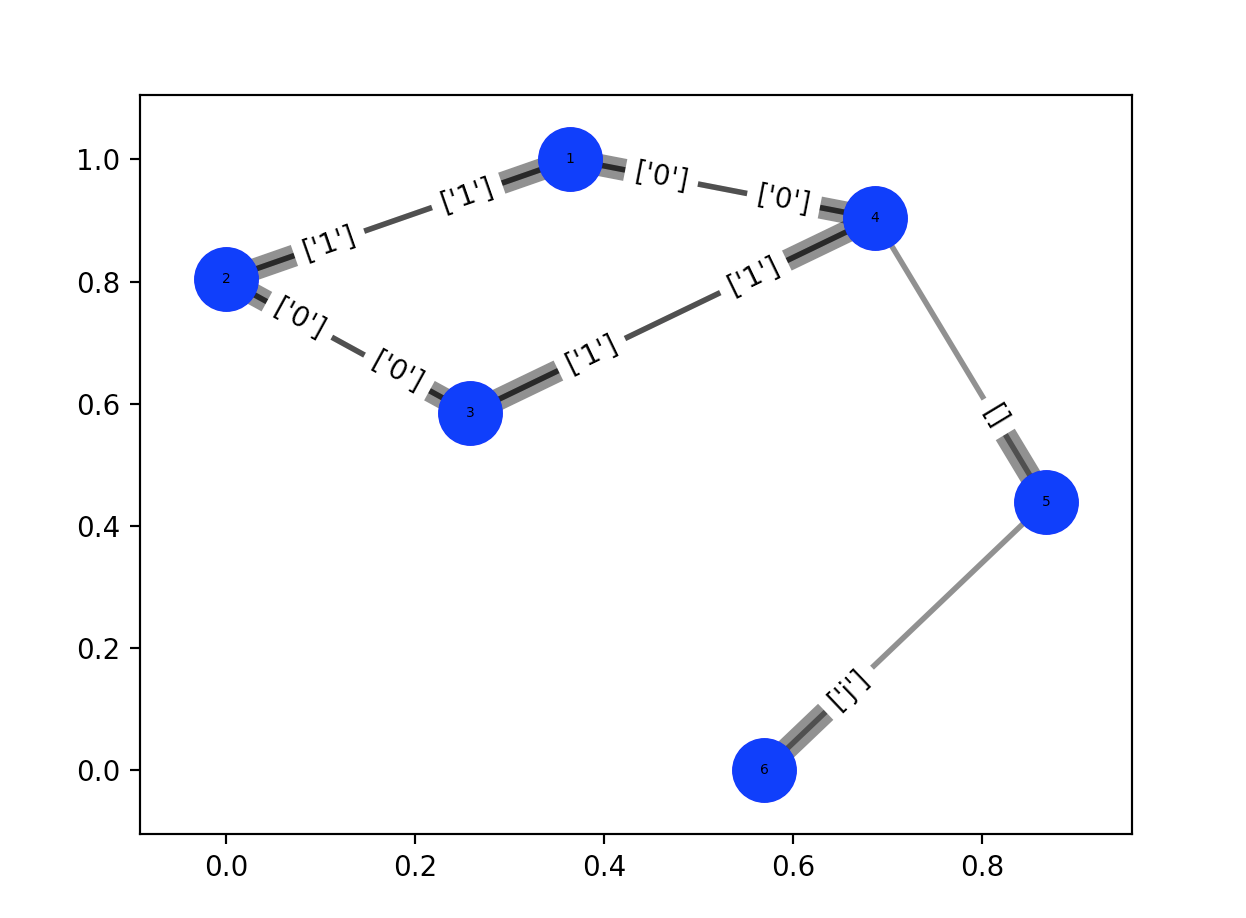
\includegraphics[width=\textwidth]{automata}
	\caption{El autómata generado.}
	\label{fig:automata}
\end{figure}

En la figura \ref{fig:resultado} se muestra el resultado de varias cadenas ingresadas al autómata generado y como retorna True si pertenecen al lenguaje modelado o False de otro modo.

\begin{figure}[H]
	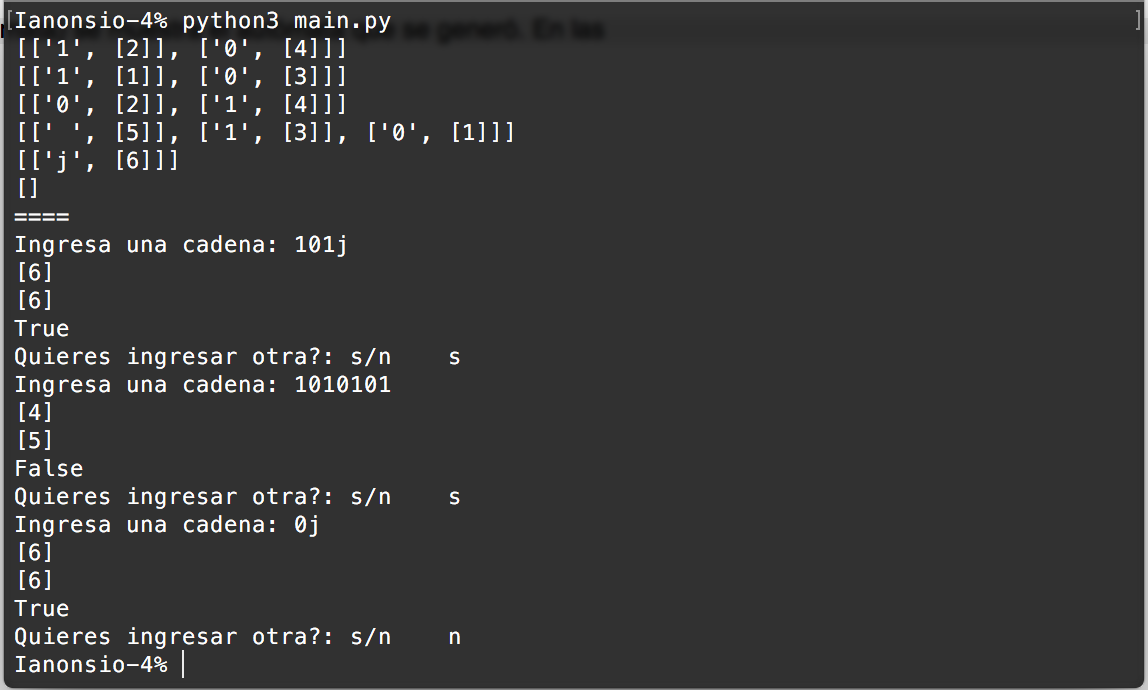
\includegraphics[width=\textwidth]{resultado}
	\caption{El resultado de varias evaluaciones.}
	\label{fig:resultado}
\end{figure}






